
\documentclass[12pt]{article}

\usepackage{sbc-template}
\usepackage{graphicx,url}
\usepackage[spanish]{babel}   
\usepackage[utf8]{inputenc}  
\usepackage{verbatim}
\usepackage{listings}
\usepackage{xcolor}
\usepackage{mips}
\usepackage{color}  

\lstset{ %
  language=[mips]Assembler,       % the language of the code
  basicstyle=\footnotesize,       % the size of the fonts that are used for the code
  numbers=left,                   % where to put the line-numbers
  numberstyle=\tiny\color{gray},  % the style that is used for the line-numbers
  stepnumber=1,                   % the step between two line-numbers. If it's 1, each line 
                                  % will be numbered
  numbersep=5pt,                  % how far the line-numbers are from the code
  backgroundcolor=\color{white},  % choose the background color. You must add \usepackage{color}
  showspaces=false,               % show spaces adding particular underscores
  showstringspaces=false,         % underline spaces within strings
  showtabs=false,                 % show tabs within strings adding particular underscores
  frame=single,                   % adds a frame around the code
  rulecolor=\color{black},       
  tabsize=4,                      % sets default tabsize to 2 spaces
  captionpos=b,                   % sets the caption-position to bottom
  breaklines=true,                % sets automatic line breaking
  breakatwhitespace=false,        % sets if automatic breaks should only happen at whitespace
  title=\lstname,                 % show the filename of files included with \lstinputlisting;
                                  % also try caption instead of title
  keywordstyle=\color{blue},          % keyword style
  commentstyle=\color{dkgreen},       % comment style
  stringstyle=\color{mauve},         % string literal style
  escapeinside={\%*}{*)},            % if you want to add a comment within your code
  morekeywords={*,...}               % if you want to add more keywords to the set
}

\definecolor{verde}{rgb}{0,0.5,0}
\definecolor{dkgreen}{rgb}{0,0.6,0}
\definecolor{gray}{rgb}{0.5,0.5,0.5}
\definecolor{mauve}{rgb}{0.58,0,0.82}

\lstset{language=verilog,
                belowcaptionskip=1\baselineskip,
                breaklines=true,
                frame=false,
                xleftmargin=\parindent,
                showstringspaces=false,
                basicstyle=\footnotesize\ttfamily,
                keywordstyle=\bfseries\color{green!40!black},
                commentstyle=\itshape\color{purple!40!black},
                identifierstyle=\color{blue},
                stringstyle=\color{orange},
                numbers=left,
            }

\sloppy

\title{Implementación procesador MIPS\\ Facultad de Ciencias Exactas, Físicas y Naturales}

\author{Sardoy, Juan Manuel\inst{1}, Perez, Federico\inst{1}}


\address{Arquitectura de computadoras - FCEFyN\\
  Av. Velez Sarsfield 1600 --  Córdoba -- Argentina
  \email{jmsardoy@gmail.com, 0xfede07c8@gmail.com}
}

\begin{document} 

\maketitle

\begin{resumen}
  Este documento describe, de manera sintética, la implementación práctica del pipeline de un procesador que cumple con un subconjunto del set de instrucciones de la arquitectura MIPS IV de 32 bits. La implementación está basada en tecnologia FPGA, mediante el lenguaje Verilog. Este trabajo tiene como objeto el aprendizaje de los diferentes elementos más comunes de la arquitectura de computadoras, dado el encuadre académico del mismo.\\
  \textbf{Palabras clave}: MIPS, FPGA, pipeline.
\end{resumen}

\begin{abstract}
  This document describes, in a synthetic way, a practical implementation of the pipeline of a processor that is compliant with a subset of the MIPS IV 32bits architecture instruction set. This job has as objective, to build the basic knowledge of the computer's architecture cope of study. \\
  \textbf{Keywords}: MIPS, FPGA, pipeline.
\end{abstract}

\section{Introducción}

El trabajo, se encuentra dentro del marco de la asignatura de Arquitectura de Computadoras, de la FCEFyN de la Universidad Nacional de Córdoba, Argentina. Corresponde al trabajo final de la misma, el cual es requerimiento para su aprobación. 

Además de la implementación del procesador en sí, se mostrará como implementar los elementos auxiliares requeridos para su funcionamiento y programación, entre otras utilidades. El hardware utilizado será un dispositivo FPGA, de la marca Xilinx, al ser de esta empresa, con los que cuentan los autores del trabajo. 

Dentro de los elementos auxiliares, encontraremos el desarrollo de un sistema de comunicación directo con el procesador, mediante el protocolo UART. Además de éste, un mecanismo para cargar un programa en la RAM del procesador, como asi también funcionalidad de debugging (ejecución paso a paso y salída de valores de registros internos). También se mostrará la implementación y uso de software auxiliar para el ensamblado de los programas a ejecutar. 

Todo esto compondrá una suite básica de desarrollo de software de propósito general, cuyo entendimiento es el objetivo principal del trabajo y la materia.


\section{Referencias Teóricas} \label{sec:firstpage}

La técnica de \textit{pipeline} es la más común utilizada para la implementación de procesadores modernos de diferentes arquitecturas, dado el gran aumento de \textit{IPC} (instrucciones por ciclo) que éste provee.

MIPS son las siglas de /textit{Microprocessor without interlocked pipeline stages}. Es una arquitectura RISC (\textit{reduced instruction set computer} desarrollada por MIPS Computer Systems. Existen versiones de 32 y 64 bits de dicha arquitectura. La primera versión de fue desarrollada en la Universidad de Stanford en 1981 por un equipo liderado por John. L. Hennesy. La idea era diseñar un procesador segmentado (idea ya muy conocida en esos momentos) pero sin interbloqueo entre capas. En esa época eran comunes los procesadores donde cada instrucción iba ejecutandose por cada capaz, mientras las otras permanecian inactivas. Esto llevaba a que el tiempo que demora en ejecutar la instrucción fuera el del tiempo en el que tarda en pasar por todas las capas, en contraste con el tiempo del camino crítico, como ocurre sin interbloqueo. 

Por estos motivos este trabajo tendrá como cuerpo principal, la aplicación de dicha técnica, para lo cual, a modo de guía, se seguirá la bibliografía de \textit{Patterson y Hennesy}, dado que expone y soluciona los problemas más comunes a la hora de la creación de un \textit{pipeline} genérico. Sin embargo, muchas partes de la implementación, quedan a cargo, y serán solucionadas por los autores, lo cual lo hace una implementación única de la arquitectura.

\section{Metodología}

Se utilizará una metodología incremental y modular para la implementación del pipeline y sus módulos complementarios. Esto mejora el entendimiento y fragmentación del problema, asi como también facilta su implementación, dado la complejidad del mismo. También esto es muy util a la hora del testing y el debugeado del sistema.

\section{Requerimientos del trabajo}\label{sec:consigna}

Los requerimientos provistos por la cátedra fueron los siguientes:

\begin{enumerate}
  \item Implementar el pipeline de un procesador MIPS, segmentado en las siguientes etapas:
  \begin{enumerate}
    \item \textbf{IF} (Instruction Fetch): Búsqueda de la instrucción en la memoria de programa.
    \item \textbf{ID} (Instruction Decode): Decodificación de la instrucción y lectura de registros.
    \item \textbf{EX} (Excecute): Ejecución de la instrucción propiamente dicha.
    \item \textbf{MEM} (Memory Access): Lectura o escritura desde/hacia la memoria de datos.
    \item \textbf{WB} (Write back): Escritura de resultados en los registros.
  \end{enumerate}
  \item En dicha arquitectura, implementar las siguientes instrucciones:
  \begin{enumerate}
    \item \textbf{R-type} (SLL, SRL, SRA, SLLV, SRLV, SRAV, ADDU, SUBU, AND, OR, XOR, NOR, SLT?
    \item \textbf{I-Type} (LB, LH, LW, LWU, LBU, LHU, SB, SH, SW, ADDI, ANDI, ORI, XORI, LUI, SLTI, BEQ, BNE, J, JAL)
    \item \textbf{J-Type} (JR, JALR)
  \end{enumerate}
  \item Debe poseer soporte (detección y manejo) de los siguientes tipos de riesgos:
  \begin{enumerate}
    \item \textbf{Estructurales}: Cuando dos o más instrucciones tratan de utilizar el mismo recurso en el mismo ciclo.
    \item \textbf{Datos}: Una etapa desea utilizar un dato antes de que esté listo. Se debe mantener el orden estricto de las lecturas y escrituras. 
    \item \textbf{Control}: Capacidad para tomar una decición sobre una condicion no evaluada. \\
    Para esto debe implementar:
    \item \textbf{Unidad de detección} riesgos: Detecta los posibles riesgos de cada tipo, y efectua los controles necesarios.
    \item \textbf{Unidad de cortocircuitos}: Ayuda en el transpaso de datos de una etapa a otra, de ser requeridos inmediatamente. Elimina la necesidad de que los datos lleguen a la última etapa de escritura de registros para que estos sean usados por otros. 
  \end{enumerate}
      \item \textbf{Ensablador:} Debe implementarse un programa ensamblador, en el cual dado una entrada en assembler de MIPS, se obtenga una salida de código máquina, apto para ser ejecutado.
      \item \textbf{Unidad de Debug:} Administra y monitorea la ejecución del procesador mediante una interfaz UART. Debe ser capaz de cargar un programa en memoria, correrlo en varios modos, y mostrar el estado del procesador. \\ \\
      \textit{Los datos que se deben envíar son:} \\
      \begin{enumerate}
        \item Contenido de los 32 registros.
        \item Contenido de los latches intermedios.
        \item Program counter.
        \item Contenido de la memoria de datos.
        \item Cantidad de clocks desde el inicio. \\
      \end{enumerate}
      \textit{Los modos de operación que debe soportar son:} \\

      \begin{enumerate}
        \item \textbf{Continuo:} Una vez cargado el programa, se envía un comando que comienza la ejecución del mismo. Al terminar, se envía la información del estado del procesador.
        \item \textbf{Paso a paso:} Se comienza con la ejecución, pero esta vez, con cada comando, se ejecuta un ciclo del clock, y se envía la informacion del estado del procesador. \\
      \end{enumerate}

      Además de estos requerimientos, los autores, a modo de mejoras, incluyen los siguientes: \\

      \item \textbf{Interfaz gráfica WEB para el debugger:} Desde esta interfaz se puede cargar un programa, ejecutarlo e inspeccionar los resultados.
      \item \textbf{Tests automatizados}: Capacidad de correr una tanda de tests sobre la implementación del MIPS y obtener un resumen de los resultados obtenidos. Esto sirve para corroborar el funcionamiento del procesador, y también que los cambios aplicados no modifiquen el comportamiento correcto comportamiento del mismo. Nótese que estos test no son lo mismo que un \textit{test bench} de Verilog. La diferencia entre ambos es que unos son simulaciones del diseño, y el otro sobre el procesador ya sintetizado. 
\end{enumerate}

\section{Pipeline de cinco etapas: Descripción general}

En la (Figura~\ref{fig:pipeline}) se puede apreciar un diagrama simplificado y general del sistema que compone a un procesador segmentado en cinco etapas. En las siguientes sub-secciones se explicará cada una de ellas. Más adelante se agregará complejidad a éste diagrama, dado los problemas que irán surgiendo y su solución.

\begin{figure}[ht]
\centering
\hspace*{-1cm} 
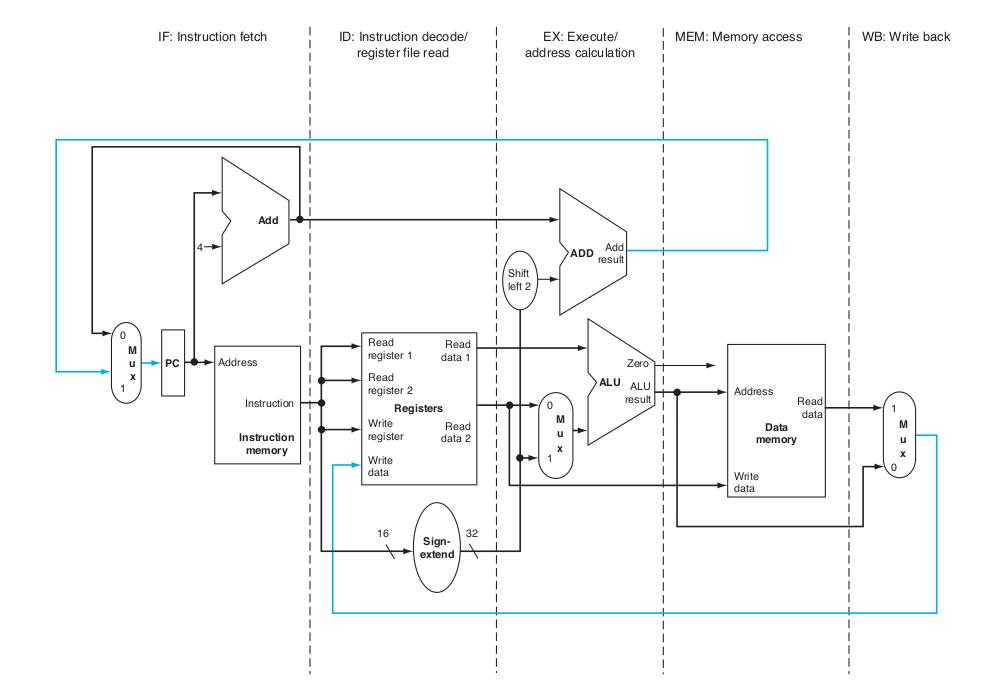
\includegraphics[width=1.1\textwidth]{imagenes/esquema_pipeline.jpeg}
\caption{Pipeline de cinco etapas: Diagrama \cite{patterson}}
\label{fig:pipeline}
\end{figure}

\subsection{\textit{IF o Instruction Fetch}} 
Es la primer etapa del pipeline. Se busca la siguiente instrucción a ejecutar en la memoria de programa. En ésta etapa se ubica el contador de programa o /textit{Program Counter}, mejor conocido como PC, el cual es un registro que contiene la dirección actual en la memoria de programa en la que se encuentra el programa en ejecución. La siguiente instrucción a ejecutar antes del ciclo es PC + WORD\_SIZE (4 para un procesador de 32bits), en caso que no haya un salto. Para mejor claridad, los pasos que ocurren en el ciclo son:

\begin{enumerate}
    \item Se calcula el nuevo valor de PC. Para eso existe un multiplexor a la entrada del PC que toma el valor desde dos fuentes. La primera es el módulo sumador, que simplemente devuelve la siguiente instrucción, y la otra fuente es una dirección arbitraria que viene desde la etapa de ejecución, producto de una instrucción de salto, condicional o absoluta.
    \item Con el valor del PC se accede a la memoria de programa, se obtiene el valor en dicha dirección, y se entrega a la siguiente etapa.
\end{enumerate}

\subsection{\textit{ID o Instruction Decode}} 
Etapa en donde se decodifica la instrucción y se cargan los registros correspondientes. Aqui tiene lugar el File Register, el módulo encargado de contener los 32 registros de 32bits del MIPS. Cada instrucción se transforma en sus correspondientes señales en la Unidad de Control, el cual comanda todo el procesador, según que instrucción se esté ejecutando. 

\subsection{\textit{EX o Excecute}} 
Unidad que ejecuta la instrucción, osea, que efectua el cálculo aritmético, lógico, o de resolución de dirección de offset. Vemos que una entrada de la ALU de propósito general puede ser un valor inmediato, con el signo extendido, o un registro, mientras que la otra entrada es siempre un registro. Existe otra ALU que unicamente suma, la cual cálcula nuevas direcciones para el PC, el cual le suma a éste un valor inmediato, el cual corresponde al salto a efectuar.

\subsection{\textit{MEM o Memory Access}} 
Unidad de lectura o escritura desde/hacia la memoria de datos. En ésta etapa se lee o escribe un dato de la memoria de acuerdo a la instrucción ejecutada. Si la instrucción no es de acceso a memoria, se hace un bypass de ésta etapa hacia la siguiente.

\subsection{\textit{WB o Write back}} 
Escritura de resultados en los registros. Los registros pueden ser escritos desde un dato en memoria, si la instrucción era de acceso a memoria, o desde la ALU si no lo eran. Se llama Write Back porque escriben sobre una etapa anterior del pipeline.

\section{Pipeline de cinco etapas: Problema completo}

El primer pipeline presentado, es simple, funciona y expone correctamente la teória básica de la segmentación en el diseño de un procesador, lo cual es necesario para el marco de éste trabajo, pero presenta problemas muy grandes, que de no ser solucionados, prácticamente elimina las ventajas del pipeline debido a su ineficiencia a la hora de enfrentar ciertos casos comunes.

El presente trabajo no planea ser una explicación teórica de todas las técnicas utilizadas y los problemas resueltos, por eso se irá al grano de la implementación completa, pero dejando al lector la posibilidad de consultar la bibliografía en el caso de ser necesario. Sin embargo, se explicará brevemente el motivo de cada uno de los elementos incluidos en el mismo.

Un esquema aproximado de la implementación completa del pipeline es el de la (Figura~\ref{fig:pipelinecompleto}).

\begin{figure}[ht]
\centering
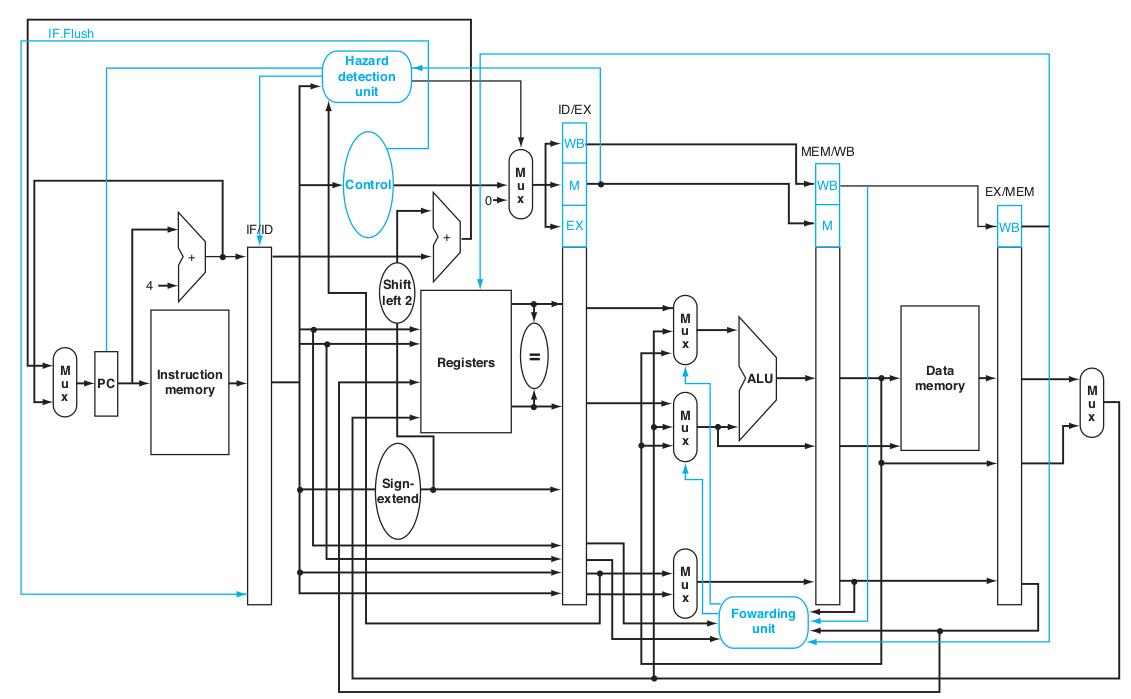
\includegraphics[width=.9\textwidth]{imagenes/esquema_pipeline_completo.jpeg}
\caption{Pipeline de cinco etapas completo \cite{patterson}}
\label{fig:pipelinecompleto}
\end{figure}


Podemos ver como se agregan diferentes unidades y complejidad que resuelven problemas determinados. Los mas significativos son los latches intermedios \textit{etapa-1/etapa}, la unidad de detección de riesgos o \textit{hazard detection unit}, la unidad de control, la unidad de forwarding, y en nuestro caso, la unidad de saltos o \textit{branching unit}. A continuación se hablara de cada una de esas unidades, explicando brevemente el funcionamiento de las mismas.

\subsection{Latches intermedios}

Las etapas deben pasarse datos unas a las otras, y mas de una vez, una etapa debe obtener datos de mas de una etapa anterior a ella misma. Si una etapa deseara hacer esto, sin interbloqueo, le resultaría imposible, dado que el estado de una etapa anterior ya ha cambiado con respecto a la instrucción que le corresponde. Por este motivo se incluyen registros o latches intermedios entre cada etapa, que almacenan los datos necesarios para el flujo del pipeline. Sirven de buffer general a las señales que se deseen conservar.

Estos latches se nombran de acuerdo a las etapas que unen. Por ejemplo, el registro que une la etapa IF con la etapa ID se llama IF/ID.

\subsection{Hazard detection unit}

Para explicar qué hace esta unidad tenemos que analizar algunos conceptos teóricos:

\subsubsection{Dependencias}

Veamos que ocurre cuando una instrucción necesita un dato de una instrucción inmediatamente anterior:

\begin{lstlisting}
sub   $2, $1,$3
and   $12,$2,$5
or    $13,$6,$2
add   $14,$2,$2
sw    $15,100($2)
\end{lstlisting}



\begin{table}[!ht]
\centering
\caption{Exemplo de tabela de 3 colunas e 2 linhas}
\label{tab:exTable1}
\smallskip
\begin{tabular}{l c c}
\hline
& Value 1 & Value 2\\[0.5ex]
\hline
&&\\[-2ex]
Case 1 & 1.0 $\pm$ 0.1 & 1.75$\times$10$^{-5}$ $\pm$ 5$\times$10$^{-7}$\\[0.5ex]
\hline
&&\\[-2ex]
Case 2 & 0.003(1) & 100.0\\[0.5ex]
\hline
\end{tabular}
\end{table}

\subsection{Código fonte}
A inserção de código fonte deve ser por meio

\begin{lstlisting}

int main(){
  int a,b,c;
  float x;
  printf("informe o tamanho do lado do quadrado");
  scanf("%d", &a);
  printf("A area do quadrado %d", b=area(a));
  printf("Duas vezes o valor do lado do quadrado %d", c=aumenta(a));

\end{lstlisting}



\section{Considerações Finais}

Referências bibliográficas devem ser utilizadas dentro de um estilo uniforme e não ambíguo. A SBC sugere os seguintes formatos para referências: \cite{patterson} \cite{instructionset}.

\bibliographystyle{sbc}
\bibliography{sbc-template}

\end{document}
